% -*- root: article.tex -*-
\subsection{Percepção dos Desenvolvedores}

\begin{figure*}
\centering
\begin{subfigure}{.22\textwidth}
  \centering
  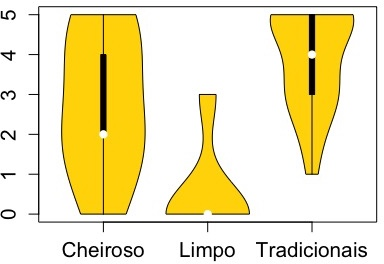
\includegraphics[width=1\textwidth]{plot-lcui-violin3.jpg}
  \caption{LCUI}
  \label{fig:lcui}
\end{subfigure}%
\begin{subfigure}{.17\textwidth}
  \centering
  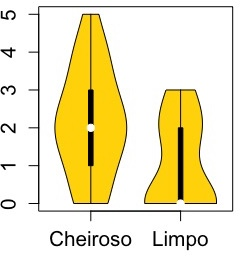
\includegraphics[width=.85\textwidth]{plot-recursos-violin2.jpg}
  \caption{Integrados}
  \label{fig:resources}
\end{subfigure}%
\begin{subfigure}{.17\textwidth}
  \centering
  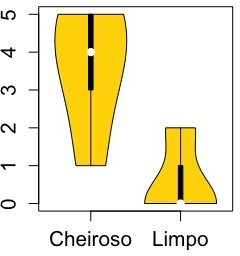
\includegraphics[width=.85\textwidth]{plot-lpa-violin2.jpg}
  \caption{LPA}
  \label{fig:lpa}
\end{subfigure}% 
\begin{subfigure}{.17\textwidth}
  \centering
  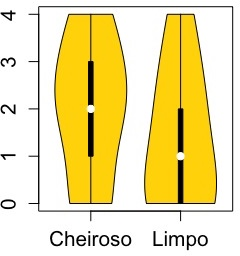
\includegraphics[width=.85\textwidth]{plot-rm-violin.jpg}
  \caption{RM}
  \label{fig:rm}
\end{subfigure}
\begin{subfigure}{.17\textwidth}
  \centering
  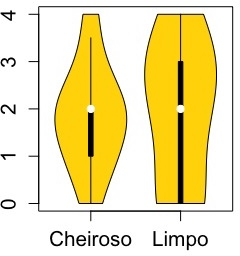
\includegraphics[width=.85\textwidth]{plot-nrd-violin.jpg}
  \caption{NRD}
  \label{fig:nrd}
\end{subfigure}% 
\caption{Gráficos violino individuais das más práticas que afetam recursos (LPA, RM e NRD).}
\label{fig:all-resources}
\vspace{-.7cm} 
\end{figure*}


As Figuras \ref{fig:lcui} e \ref{fig:all-resources} apresentam gráficos de violino sobre a percepção dos desenvolvedores com relação as quatro más práticas de alta recorrência (LCUI, LPA, RM e NRD). 

No eixo y, 0 (zero) indica códigos não percebidos pelos desenvolvedores como problemáticos (ou seja, responder \emph{não} à pergunta: este código apresenta algum problema de design e/ou implementação?), enquanto que valores de 1 a 5 indicam o nível de severidade para o problema percebido pelo desenvolvedor.

\subsubsection{Más práticas que afetam classes Java}
% \begin{figure}
% 	\centering
% 	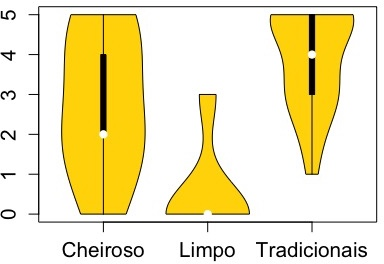
\includegraphics[width=0.3\textwidth]{plot-lcui-violin3.jpg}
% 	\caption{LCUI}
% 	\label{fig:lcui}
% \end{figure}

Na Figura \ref{fig:lcui} apresentamos três gráficos violinos, respectivamente: percepção dos desenvolvedores sobre códigos afetados pela má prática LCUI, a percepção sobre códigos limpos e por último, a percepção sobre códigos afetados por maus cheiros tradicionais como por exemplo Classe Longa. 

A mediana de classes limpas tem severidade igual a 0 (Q3=0). Isso indica que, como esperado, desenvolvedores não percebem essas classes como problemáticas. Em comparação, as classes afetadas por LCUI tem mediana igual a 2 (Q3=4) logo, são percebidas como classes problemáticas. A diferença entre classes afetadas por LCUI e classes limpas é estatisticamente significante (p-value < 0.004) com alto tamanho de efeito (d = 0,72). Com relação aos maus cheiros tradicionais, a mediana de severidade é igual a 4 (Q3=5). Isso significa que classes afetadas por esses maus cheiros são percebidas pelos desennvolvedores como muito problemáticas, ainda mais que classes afetadas pela má prática em questão. Ainda que essa diferença de percepção esteja clara no gráfico violino, esta diferença não é estatisticamente significante (p-value = 0.077). Acreditamos que isso ocorra devido ao número limitado de dados (20 participantes).

% LCIU p-value e d completos/originais/sem quebrar decimal
% Notamos que, desenvolvedores de fato percebem classes afetadas pela má prática LCUI como problemáticas (p-value 0.003045 e d 0.7222222 (large)). Bem como, classes afetadas por maus cheiros tradicionais também são percebidas como problemáticas (p-value 6.367e-06 e d -0.9130435 (large)). Porém, não podemos afirmar se, maus cheiros tradicionais são considerados mais ou menos importantes do que a má prática LCUI (p-value 0.07667 e d -0.3961353 (medium)). Ao observar as respostas abertas, a maioria dos participantes pontuou a questão de haver lógica na classe de \textit{front-end}, que é o ponto central desta má prática, como o problema. Podemos citar S2P11 que diz ``\textit{[...] Não há nenhuma arquitetura implementada, o que causa a classe fazendo muito mais do que é de sua alçada. O método onListItemClick está muito complexo, contendo 7 condições [...]}''.

\subsubsection{Más práticas que afetam recursos}

A Figura \ref{fig:all-resources} reúne 4 diferentes pares de gráficos violinos. O primeiro compara recusos afetados por quaisquer das 3 más práticas, LPA, RM e NRD, com recursos limpos. O segundo, terceiro e quarto, trata de cada má prática individualmente, ou seja, recursos afetadas por aquela má prática em comparação com recursos limpos. 

A Figura \ref{fig:resources} mostra a percepção dos desenvolvedores com relação a recursos afetados pelas más práticas LPA, RND e RM, com mediana de severidade igual a 2 (Q3=3), em comparação com recursos limpos (mediana igual a 0). Isso indica que, como esperado, desenvolvedores percebem recursos afetados pelas más práticas como problemáticos. Essa diferença também é estatisticamente significante (p-value < 0.008) com médio tamanho de efeito (d = 0.43).

% XMLS vs LIMPOS dados completos
% podemos observar que, de fato, desenvolvedores percebem, de forma geral, recursos afetados pelas más práticas LPA, RM ou NRD, como problemáticos (p-value 0.007986 e $\delta$ 0.4335664 (medium)). 

Ao avaliarmos os gráficos violinos das más práticas individualmente, podemos notar que duas, LPA (Figura \ref{fig:lpa}) e RM (Figura \ref{fig:rm}), se mostram percebidas como problemáticas, sendo a primeira mais percebida do que a segunda. Códigos afetados pela má prática LPA tem mediana de severidade igual a 4 (Q3=5) logo, desenvolvedores percebem códigos afetados por ela como problemáticos. Em comparação, código limpos apresentam mediana 0 (Q3=1). A diferença entre códigos afetados por LPA e códigos limpos também é estatisticamente significante (p-value < 0.02) com alto tamanho de efeito (d = 0,89). Em contrapartida, ainda que o gráfico de violino da má prática RM apresente também uma diferença visual entre códigos limpos e afetados pela má prática, essa diferença não é estatisticamente significante (p-value = 0,34).

A má prática NRD foi a menos percebida por desenvolvedores, com medianas iguais para códigos afetados por ela e códigos limpos (mediana = 2). Entretando, os desenvolvedores que indicaram códigos afetados por ela como problemáticos, indicaram como o problema descrições muito próximas a definição dada para essa má prática. Por exemplo, S2P15 disse ``\textit{Os nomes das strings são formados por um prefixo e um número, o que prejudica a legibilidade, é impossível saber o que este número indica}'' (pontuou severiadade como 3), S2P16 disse ``\textit{Atributos não seguem convenção de nomes. Nomes não são descritivos}'' (pontuou severiadade como 2), S2P11 disse ``\textit{Não segue uma boa prática de nomenclatura de recursos.}'' (pontuou severiadade como 2) e S2P19 disse ``\textit{Os nomes das strings não estão seguindo um padrão (algumas em camelCase, outras lowercase, outras snakecase) [...]}'' (pontuou severiadade como 2). Algumas possíveis ideias que justificariam esse resultado são discutidas na Seção \ref{discussao}. \\

De forma geral, os desenvolvedores conseguiram identificar corretamente a má prática em questão, colocando em suas respostas descrições muito próximas as definições dadas a elas. Por exemplo S2P11 ao confrontar um código afetado por LCUI disse ``\textit{[...] Não há nenhuma arquitetura implementada, o que causa a classe fazendo muito mais do que é de sua alçada. O método onListItemClick está muito complexo, contendo 7 condições [...]}'', S2P5 ao confrontar um código afetado por RM disse ``\textit{Valores de cores, tamanhos, animaçoes e distancias, nao estao extraidos fazendo que muitos deles estejam repetidos dificultando uma posterior manutençao ou reusabilidade}'', S2P7 ao confrontar um código afetado por LPA disse ``\textit{Os sucessivos aninhamentos de view groups provavelmente irá causar uma performance ruim}''.

% \begin{figure*}
% \centering
% \begin{subfigure}{.19\textwidth}
%   \centering
%   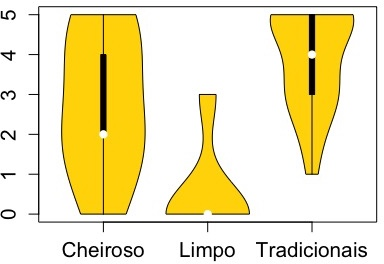
\includegraphics[width=1.1\textwidth]{plot-lcui-violin3.jpg}
%   \caption{LCUI}
%   \label{fig:lcui}
% \end{subfigure}%
% \begin{subfigure}{.19\textwidth}
%   \centering
%   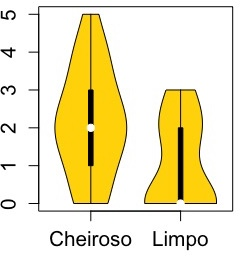
\includegraphics[width=.7\textwidth]{plot-recursos-violin2.jpg}
%   \caption{Integrados}
%   \label{fig:resources}
% \end{subfigure}%
% \begin{subfigure}{.19\textwidth}
%   \centering
%   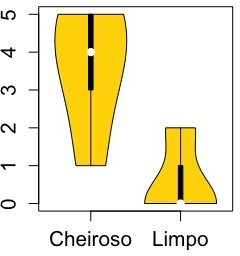
\includegraphics[width=.7\textwidth]{plot-lpa-violin2.jpg}
%   \caption{LPA}
%   \label{fig:lpa}
% \end{subfigure}% 
% \begin{subfigure}{.19\textwidth}
%   \centering
%   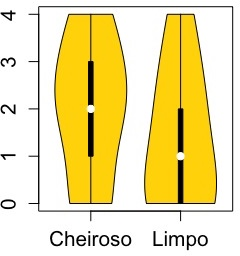
\includegraphics[width=.7\textwidth]{plot-rm-violin.jpg}
%   \caption{RM}
%   \label{fig:rm}
% \end{subfigure}
% \begin{subfigure}{.19\textwidth}
%   \centering
%   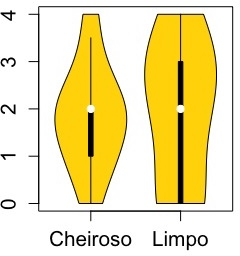
\includegraphics[width=.7\textwidth]{plot-nrd-violin.jpg}
%   \caption{NRD}
%   \label{fig:nrd}
% \end{subfigure}% 
% \caption{Gráficos violino individuais das más práticas que afetam recursos (LPA, RM e NRD).}
% \label{fig:all-resources}
% \end{figure*}











